\subsubsection{Protocolo de Comunicação via Rádio Frequência}

O protocolo utilizado no link de rádio frequência criado será o MAVLink - \textit{Micro Air Vehicle Message Marshalling Library} - é uma biblioteca de comunicação para 
pequenas quantidades de dados entre aeronaves não tripuladas e estações de controle em terra. 
Permitindo o envio de pacotes de informações através de \textit{byte-level serialization} o que torna 
compatível com qualquer onda de radio.\cite{mavlink}

Uma vez que a área de atuação do EmerVant é a Esplanada dos Ministérios, 
definido na seção \ref{escopo} - Escopo, a viabilidade e eficiência na implantação desse protocolo é
extremamente alta. Aonde o sinal emissor será posicionado na torre de TV cobrindo toda a 
área de atuação com um boa qualidade de sinal. 

\subsubsection{Protocolo de perda de sinal}

\begin{itemize}
  \item Protocolo de erros

  Para um funcionamento seguro é necessário ter em mente que podem vir a existir condições adversas as planejadas. Tendo isso em vista foi estabelecido um protocolo de erros para situações que podem vir a ocorrer durante um voo do VANT.

  \item Perda de sinal
  
  Em caso de perda de sinal o VANT deverá retornar a seu ponto de origem imediatamente.

  \item Bateria fraca

  Ao chegar em 25\% restante de bateria o VANT irá retornar para a central imediatamente.

  \item Perda de potência

  Em caso de perda de potência por parte do motor, o VANT procurará um local para pousar imediatamente.
\end{itemize}

\subsubsection{Especificação do Projeto da Comunicação do Vant}

\begin{itemize}
 \item Piloto automático guiará o VANT até a emergência: 

  A central receberá a solicitação do veículo e com as orientações do local do acidente, ela irá mapear o percurso a ser seguido para chegar até o destino.  Essas informações referentes ao trajeto e coordenadas de GPS serão passadas de forma wireless serialmente para o sistema e controladores do VANT. Para que isso aconteça, eles estarão conectadas por um canal de comunicação de radiofrequência. 

  \item Comunicação e transmissão de dados:

   A central necessitará passar informações ao usuário referentes ao atendimento, também precisará ver o estado do paciente e ver se os procedimentos foram realizados conforme as instruções e as informações dos sinais vitais da vítima para entender a real situação dele. 

\end{itemize}

\subsubsubsection{Comunicação com o Pixhawk}
O controle e configura\c{c}\~ao do voo do VANT \'e gerenciado pelo \textit{Ground Control Station}, em português, 
esta\c{c}\~ao de controle em solo. Devido à facilidade na customização e a compatibilidade com a placa controladora adotada pelo projeto, Pixhawk, foi escolhido o GCS Mission Planner mantido pelo projeto \textit{open-source  APM autopilot}.\cite{gcs}

A escolha foi feita com base na comparação entre os requisitos da aplicação descritos no documento de visão e as características dos softwares de mercado pesquisados.

Foram analisados os seguintes softwares: 

\begin{itemize}
  \item QGroundControl
  \item Mission Planner
  \item APMPlanner
\end{itemize}

Após a analise foram observados os itens da Figura \ref{fig:gcstable}

\begin{figure}[h!]
    \centering
      \includegraphics[keepaspectratio=true,scale=0.5]{figuras/gcstable.eps}
    \caption{Resultado da análise dos softwares de GCS.}
    \label{fig:gcstable}
\end{figure}

Pela Figura \ref{fig:gcstable}, pode-se perceber que o software Mission Planner é a melhor solução para o gerênciamento do VANT. Uma vez que o projeto está sob uma licença aonde é permitido o uso para comercialização, este será utilizado com GCS do VANT.

Com a utilização do \textit{GCS Mission Planner}, o processo da operação de socorro é automatizado. 
Uma vez que, com a aplicação é possível a criação de planos de voos. 
A figura \ref{fig:planovoo} mostra um exemplo de plano de voo. 
Nesse plano, o VANT decola do ponto \textit{Home}, em seguida é direcionado até ao ponto 2 e depois 
se desloca ao ponto 3 e retorna ao ponto inicial.

\begin{figure}[h!]
    \centering
	    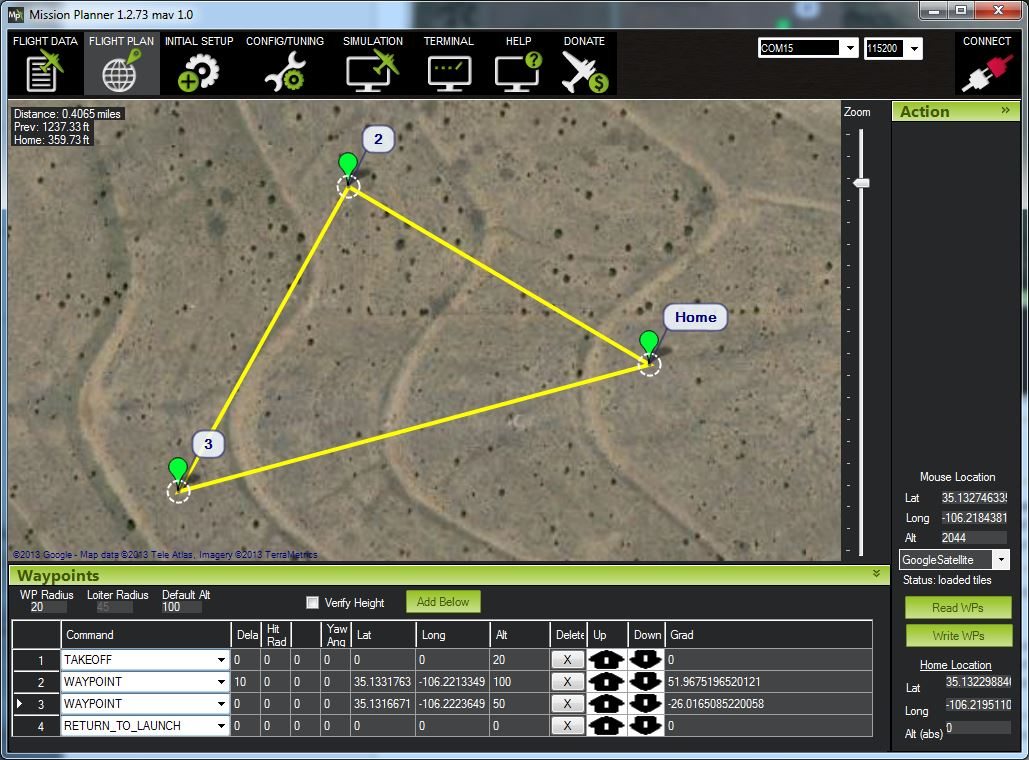
\includegraphics[keepaspectratio=true,scale=0.5]{figuras/planovoo.eps}
    \caption{Exemplo de missão da GCS. Fonte: Software \textit{Mission Planner}}
    \label{fig:planovoo}
\end{figure}


Os locais onde deve-se passar, ou pousar, ou executar um comando são definidos através das coordenadas de longitude e latitude. Assim quando ocorrer uma emergência, a equipe de controle, com o auxílio da API Google Maps integrada com o GCS, apontará as coordenadas aonde o VANT deve pousar para executar o socorro. 
A figura \ref{fig:esplanada} mostra uma missão na Esplanada dos Ministérios.

\begin{figure}[h!]
    \centering
	    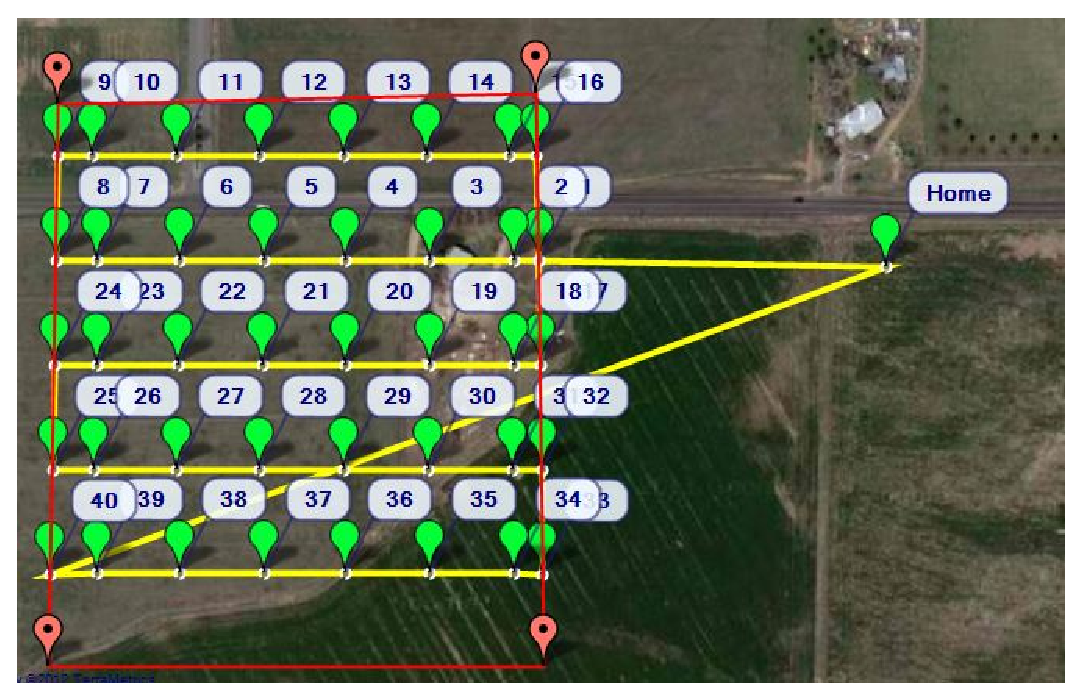
\includegraphics[keepaspectratio=true,scale=0.8]{figuras/esplanada.eps}
    \caption{Simulação feita na Esplanada. Fonte: Software \textit{Mission Planner}}
    \label{fig:esplanada}
\end{figure}

A plataforma a ser utilizado será o Microsoft Windows devido à grande utilização no Serviço Público, 
além de oferecer maior compatibilidade com os recursos utilizados, obedecendo, por exemplo, os requisitos
do sistema de comunicação com o controlador, o Mission Planner. 

\subsubsubsection{Protocolo de erros}
	
Para um funcionamento seguro é necessário ter em mente que podem vir a existir condições adversas as planejadas. Tendo isso em vista foi estabelecido um protocolo de erros para situações que podem vir a ocorrer durante um voo do VANT.

\begin{itemize}
 \item Perda de sinal: Em caso de perda de sinal o VANT deverá retornar a seu ponto de origem imediatamente.
 
 \item Bateria fraca: Ao chegar em 25\% restante de bateria o VANT irá retornar para a central imediatamente.

 \item Perda de potência: Em caso de perda de potência por parte do motor, o VANT procurará um local para pousar imediatamente.

\end{itemize}

\subsubsubsection{Comunicação do usuário com o VANT}
Nessa subseção é tratada a comunicação da central com o VANT e do cidadão com o VANT.
Nessa comunicação alguns passos devem ser seguidos, são eles:

\begin{enumerate}
  \item Uma ligação é efetuada para o sistema de emergência escolhido para a implantação dos VANT’s;
  \item O atendente da emergência avalia a situação e decide se um VANT será enviado à frente da ambulância;
  \item Caso seja necessário, o VANT será enviado e deverá chegar ao local da emergência antes da ambulância;
  \item Ao chegar ao local, uma mensagem sonora será reproduzida, pedindo que alguém se aproxime para instruções;
  Quando o VANT chegar ao local do atendimento, sua interação com o cidadão que irá socorrer o paciente se dará por intermédio de um canal de áudio (contato com o atendente) com a central, ao passo que uma câmera e microfone passarão seu áudio e vídeo para a central. 
  Apesar de analisada a possibilidade de um display no VANT para exibição de algum vídeo instrutivo, optou-se por apenas um canal de áudio para comunicação por sua simplicidade, sendo que um cidadão poderia se confundir por instruções sendo recebidas por áudio e por vídeo.
  \item Será estabelecido contato entre a central e o cidadão, sendo que este se dará de forma diferente para ambos. O atendente na central terá acesso ao aúdio e ao vídeo provenientes do local do acidente, ao passo que o cidadão terá acesso somente ao aúdio proveniente da central;
  \item Tendo sido estabelecido o contato o atendente instruirá o cidadão a posicionar o sensor no dedo do paciente para que o mesmo obtenha informações acerca do monitoramento dos sinais vitais;
  \item Se após averiguação por parte do atendente, for atestado que o paciente está sofrendo uma parada cardíaca, o cidadão será instruído a remover, de maneira respeitosa, a vestimenta superior do paciente e logo em seguida posicionar o desfibrilador presente no VANT, após feito isso será pedido que todos se afastem para que a carga do desfibrilador seja aplicada;
  \item Se após averiguação por parte do atendente, for atestado que o paciente está sofrendo uma parada respiratória, o cidadão será instruído a pegar no VANT a bomba respiratória manual e com cuidado colocar sobre o nariz do paciente, após verificar que a mesma está bem colocada e fixa no rosto do paciente, o cidadão será instruído a bombear até que a pessoa se encontre reanimada ou o socorro (ambulância) chegar;
  \item Após conclusão de todos os passos acima será solicitado pelo atendente da central que o cidadão aguarde junto ao paciente até o momento da chegada da ambulância.

\end{enumerate}
